\section{\texttt{doco}: Generating Documentation from Source Code}

In order to evaluate our goal of automatically generating documentation, we developed a tool that analyses programs written in the Java programming language. The choice for Java was based on its widespread adoption in the industry and on the fact that \texttt{doco} could build on top of existing analysis tools, developed both in industry and academia, that typically target Java.

Figure \ref{fig:flow} illustrates how \texttt{doco} performs documentation generation for a given method or function\footnote{\texttt{doco} is freely available at https://github.com/mrordinaire/doco}. In the following sections, we describe the process in greater depth and explain how we can achieve our goals by leveraging existing tools in the program analysis field.

\begin{figure}[h]
  \centering
    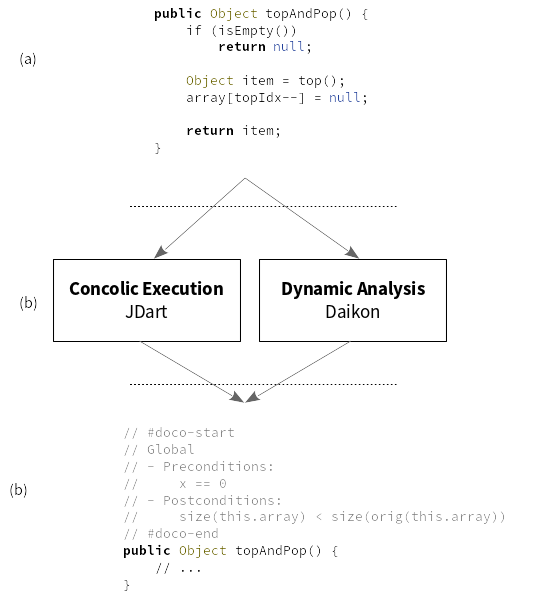
\includegraphics[width=0.4\textwidth]{doco_flow.png}
    \caption{Automatically generating documentation with \texttt{doco}. The process starts when the developer is editing a certain method on her text editor (a). When \texttt{doco} is invoked on that method, it will run static and dynamic analysis processes in parallel in order to infer invariants and properties about the method (b). Once that step is completed, the generated properties are added as comments on top of the function definition (c).}
    \label{fig:flow}
\end{figure}

\subsection{Dynamic Analysis}

Dynamic analysis is the term used to refer to analyses that are performed during the execution of a program~\cite{Ball:1999}. It works by instrumenting source code to collect usage information at a level that is granular enough to infer properties about the source code being studied.

\texttt{doco} uses the Daikon~\cite{Ernst:2007} invariant detector for its dynamic analysis module. Specifically, it invokes Daikon whenever the user wants to generate documentation for a function or method, extracts relevant invariants inferred by Daikon, and parses its results in order to generate properties that are easier for the developer to understand.

In order for the analysis to happen, the project needs to have a \textbf{test suite}. The test suite is responsible for invoking the methods of a project with both valid and invalid arguments. Daikon instruments the execution of the test suite in order to collect information about method and parameter usage.

The analysis performed by Daikon happens in two steps. In the \emph{instrumentation} phase, the test suite is executed and mediated by Daikon so that it can observe methods being called and arguments being passed to them. This step produces an intermediary representation of the execution that is stored in a file. In the \emph{inference} phase, the test suite needs to be executed again, but this time with the aid of the file created in the previous step. Daikon uses the collected data in this step to generate likely invariants for the methods it observed. Figure \ref{fig:daikon} depicts the Daikon analysis process in detail.

\begin{figure}[h]
  \centering
    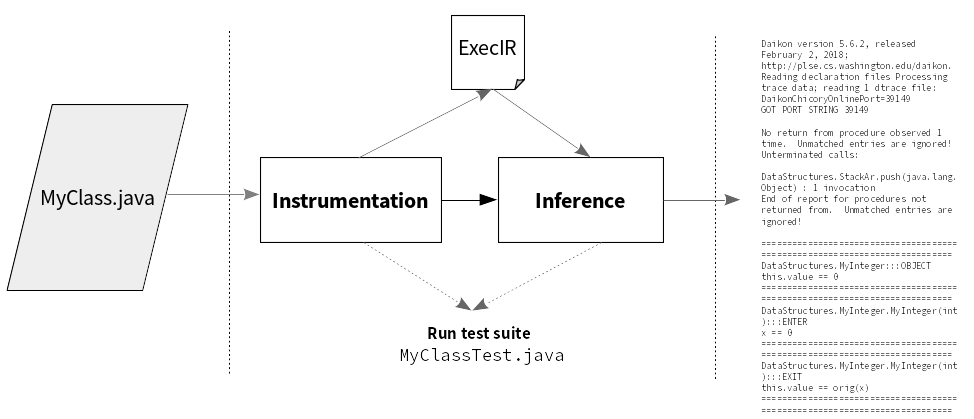
\includegraphics[width=0.4\textwidth]{daikon_flow.png}
    \caption{The steps involved in the dynamic analysis performed by Daikon. In the left, the user has a \texttt{MyClass.java} file with methods that need documentation. In the middle, Daikon infers invariants by performing a two-phase analysis of the source code based on an existing test suite. On the right, Daikon inferred properties (in the form of pre- and post-conditions) for every method invoked.}
    \label{fig:daikon}
\end{figure}

It is important to note that Daikon heavily relies on a high quality test suite in order to be able to produce pre- and post-conditions for methods. In that sense, projects with unit tests that exercise as many different kinds of arguments to every function as possible are the idead target for this kind of analysis. Luckily, that is the case for the majority of popular, open-source Java applications and libraries.

\subsection{Concolic Execution}

As mentioned in earlier, dynamic analysis requires a high quality test suite to guide analysis. This requirement constrains the quality of its results on the quality of the test suite.

Unlike dynamic analysis, concolic execution, also known as dynamic symbolic analysis, does not impose such a constraint, making it attractive for software projects with few to no tests. Concolic execution is a technique which combines dynamic and symbolic analysis. It repeatedly executes the program being analyzed both concretely, giving each variable a concrete value, and symbolically, tracking the path conditions on each variable. Having concrete values allows concolic execution to explore more deeply into the program than symbolic execution while retaining more semantic insight into the state of the program than concrete execution. Concolic execution can force execution to explore newly found path by negating path conditions previously seen. JDart~\cite{tacas2016-ldghikrr} is a concolic execution framework for Java. \texttt{doco} utilizes the method summary functionality implemented by JDart.

JDart method summary collects all the path conditions, concrete values used, as well as path results. \texttt{doco} extracts the path conditions returned by JDart, combines and simplifies them to present an easy-to-digest result to the user.

An example path condition is shown in figure~\ref{fig:pc-range}. This path condition is taken from a function that checks whether the provided argument \texttt{n} is a prime number. It is evident from the figure that simply presenting the path conditions is not enough. Therefore, \texttt{doco} tries to further simplify the output by computing the valid values a variable can take. In order to do so, \texttt{doco} represents integer variables, such as \texttt{long}, as ranges. After collecting all path conditions for paths which are OK, i.e. paths that reach the end of the method and return normally, \texttt{doco} takes the union of all the path conditions and present it to the user. 

\subsubsection{Ranges}

\begin{figure}
\centering
\begin{lstlisting}
// path condition
[L]declare 'n':sint64 in
    (('n' != 13) &&
     (('n' != 11) &&
      (('n' != 7) &&
       (('n' != 5) &&
        (('n' != 3) &&
         (('n' != 2) &&
          ('n' >= 2)))))))
// range representation
[(4, 4), (6, 6), (8, 10),
 (12, 12), (14, 9223372036854775807)]
\end{lstlisting}
\caption{An example path condition and its corresponding range representation}
\label{fig:pc-range}
\end{figure}

The values for an integer variable are represented as disjoint ranges with increasing inclusive bounds. Figure~\ref{fig:pc-range} shows an example path condition on an integer variable and its range representation. Ranges support operations such as union, intersection, and difference.

\subsection{Developer Tool Support}

Considering that developers don't prefer using static analysis tools because they are hard to set up \cite{Johnson:2013:WDS:2486788.2486877}, it was necessary to develop a front end plugin for \texttt{doco} that is integrated with a popular text editor. We chose Atom \cite{Atom} as our text editor because it offers a lot of room for customization. The \texttt{doco} plugin hides the verbose outputs from the concolic execution/dynamic analysis and presents them in the form of pre and post conditions that is easy for the user to understand. It achieves this by following a three step process after being invoked through a keyboard shortcut to generate the documentation for the user:

\begin{enumerate}
    \item \textbf{Function Identification:} As its first step towards generating documentation, \texttt{doco} identifies the function in which the user's cursor currently resides. It does this by using Atom's API to figure out where the cursor is and identifies the nearest function declaration that is above it.
    
    \item \textbf{Parsing out required inputs and configuration:} The \texttt{doco} plugin is then responsible for parsing out the function signature along with the the name of the class and the package in which the function belongs, using regular expressions. These arguments are required by JDart and Daikon to carry out their concolic execution and dynamic analysis to generate the required pre and post conditions. Moreover, the configuration information that is specified by the user and  required by these two tools e.g path to test cases for Daikon is also extracted out. The class name, function signature, package name and the configuration are then passed to each of these tools for analysis.
    
    \item \textbf{Appending documentation:} Once the concolic execution and dynamic analysis is completed, \texttt{doco} appends the generated pre and post condition above the function signature in the source code.
\end{enumerate}
